% context: markscheme (official solutions) for 2-10CW_Graphical-analysis, review
%        classwork on 19 November 2026
% topic: a labelled height-time parabola; deriving, tabulating and plotting a
%        parabola and its velocity line
% convention: answers in bold; g rounded to 10 m/s^2 throughout, so the values are
%        exact and "=" is used
\documentclass[12pt, twoside]{article}
%\documentclass[12pt, twoside]{article}
\usepackage[letterpaper, margin=1in, headsep=0.2in]{geometry}
\setlength{\headheight}{0.6in}
%\usepackage[english]{babel}
\usepackage[utf8]{inputenc}
\usepackage{microtype}
\usepackage{amsmath}
\usepackage{amssymb}
%\usepackage{amsfonts}
\usepackage[nomessages]{fp} %\FPeval{\var-name}{2*sin(pi/6)}
\usepackage{siunitx} %units in math. eg 20\milli\meter
\usepackage{yhmath} % for arcs, overparenth command
\usepackage{tikz} %graphics
\usetikzlibrary{quotes, angles, arrows, arrows.meta}
\usepackage{graphicx} %consider setting \graphicspath{{images/}}
\usepackage{parskip} %no paragraph indent
\usepackage{enumitem}
\usepackage{multicol}
\usepackage{venndiagram}

\usepackage{fancyhdr}
\pagestyle{fancy}
\fancyhf{}
\renewcommand{\headrulewidth}{0pt} % disable the underline of the header
\raggedbottom
\hfuzz=2mm %suppresses overfull box warnings

\usepackage{hyperref}
\usepackage{float}
\setlength{\parskip}{0.2\baselineskip}
\sisetup{reset-text-series=false, reset-math-version=false, text-series-to-math=true}

\title{Physics}
\author{Chris Huson}
\date{November 2026}

\fancyhead[LE]{\thepage}
\fancyhead[RO]{\thepage}
\fancyhead[LO]{La Scuola d'Italia / Huson / Physics \\* 19 November 2026}

\begin{document}

\subsubsection*{2.10 Classwork: Graphical Analysis Solutions}

\begin{enumerate}[itemsep=0.5cm]

\item \emph{Skill: motion graphs (reading a height-time graph).} Here
  $y = 40t - 5t^2$ and $v = 40 - 10t$.
  \begin{enumerate}[itemsep=0.3cm]
    \item Read from the grid lines:

      {\renewcommand{\arraystretch}{1.4}%
      \begin{tabular}{| l | c | c | c | c | c |}
        \hline
        Point & A & B & C & D & E \\ \hline
        $t$ (s) & 0 & 1 & 4 & 7 & 8 \\ \hline
        $y$ (m) & 0 & 35 & 80 & 35 & 0 \\ \hline
      \end{tabular}}
    \item \textbf{C}. \textbf{Velocity $\mathbf{v = 0}$}: the tangent there is
      flat. \textbf{Acceleration $\mathbf{a = -10}$ m/s$^\mathbf{2}$}, as at every
      other point.

      \emph{The common wrong answer is $a = 0$ at the top.}
    \item \textbf{Up from A to C}: the height increases, the slope is positive.
      \textbf{Down from C to E}: the height decreases, the slope is negative.
    \item slope $= \dfrac{80 - 0~\text{m}}{4 - 0~\text{s}} =
      \mathbf{20~\textbf{m/s}}$. \textbf{It is the average velocity on the way up.}

      \emph{It is half of 40 m/s, as $\bar{v} = \frac{v + v_0}{2} = \frac{0 +
      40}{2}$ predicts.}
    \item $v_B = 40 - 10 \times 1 = \mathbf{+30~\textbf{m/s}}$ \qquad
      $v_D = 40 - 10 \times 7 = \mathbf{-30~\textbf{m/s}}$ \qquad
      $v_E = 40 - 10 \times 8 = \mathbf{-40~\textbf{m/s}}$

      \textbf{B and D: the same speed, 30 m/s, but B is going up and D is coming
      down.} At E the rocket is back at launch height, moving at its launch speed,
      downward.

      \emph{Also accept the symmetry argument: D is as far after the top as B is
      before it.}
    \item slope $= \dfrac{35 - 35~\text{m}}{7 - 1~\text{s}} = \mathbf{0}$.
      \textbf{The average velocity from B to D is zero}: the rocket ends where it
      started, so its displacement is zero, even though it travelled
      $2 \times 45 = 90$ m.
  \end{enumerate}

\item \emph{Skill: motion graphs (plotting free fall).}
  \begin{enumerate}[itemsep=0.3cm]
    \item With $y_0 = 0$, $v_0 = 10$ m/s, $a = -10$ m/s$^2$:
      $y = y_0 + v_0 t + \frac{1}{2}at^2 = 0 + 10t + \frac{1}{2}(-10)t^2 =
      \mathbf{10t - 5t^2}$ \quad and \quad $v = v_0 + at = \mathbf{10 - 10t}$.
    \item Square the time first: at 0.6 s, $y = 10(0.6) - 5(0.36) = 6.0 - 1.8 =
      4.2$ m.

      {\renewcommand{\arraystretch}{1.4}%
      \begin{tabular}{| l | c | c | c | c | c | c | c | c | c | c | c |}
        \hline
        $t$ (s) & 0 & 0.2 & 0.4 & 0.6 & 0.8 & 1.0 & 1.2 & 1.4 & 1.6 & 1.8 & 2.0
          \\ \hline
        $y$ (m) & 0 & 1.8 & 3.2 & 4.2 & 4.8 & \textbf{5.0} & 4.8 & 4.2 & 3.2 & 1.8
          & 0 \\ \hline
        $v$ (m/s) & 10 & 8 & 6 & 4 & 2 & \textbf{0} & $-2$ & $-4$ & $-6$ & $-8$ &
          $-10$ \\ \hline
      \end{tabular}}

      \emph{The heights are symmetric about 1.0 s, which is a built-in check. The
      usual error is $0.2^2 = 0.4$.}
    \item Plotted points, a smooth curve, and a ruled line:

      \begin{tikzpicture}[x=2.65cm, y=1.2cm]
        \draw[gray!25, thin, xstep=0.1, ystep=0.2] (0,0) grid (2.0,5.6);
        \draw[gray!60, xstep=0.2, ystep=1] (0,0) grid (2.0,5.6);
        \draw[->, thick] (0,0) -- (2.1,0) node[below right]{\small $t$ (s)};
        \draw[->, thick] (0,0) -- (0,5.8) node[above]{\small $y$ (m)};
        \foreach \t in {0,0.4,0.8,1.2,1.6,2.0} \node[below] at (\t,0) {\scriptsize \t};
        \foreach \y in {1,...,5} \node[left] at (0,\y) {\scriptsize \y};
        \draw[very thick, domain=0:2, samples=60] plot (\x, {10*\x - 5*\x*\x});
        \foreach \t in {0,0.2,...,2.0} \fill (\t, {10*\t - 5*\t*\t}) circle (1.8pt);
      \end{tikzpicture}
      \hfill
      \begin{tikzpicture}[x=2.65cm, y=0.335cm]
        \draw[gray!25, thin, xstep=0.1, ystep=1] (0,-10) grid (2.0,10);
        \draw[gray!60, xstep=0.2, ystep=2] (0,-10) grid (2.0,10);
        \draw[->, thick] (0,0) -- (2.1,0) node[above right]{\small $t$ (s)};
        \draw[->, thick] (0,-10) -- (0,11) node[above]{\small $v$ (m/s)};
        \foreach \t in {0.4,0.8,1.2,1.6,2.0}
          \node[below, fill=white, inner sep=1pt] at (\t,-0.3) {\scriptsize \t};
        \foreach \v in {-10,-8,-6,-4,-2,2,4,6,8,10}
          \node[left] at (0,\v) {\scriptsize \v};
        \draw[very thick] (0,10) -- (2,-10);
        \foreach \t in {0,0.2,...,2.0} \fill (\t, {10 - 10*\t}) circle (1.8pt);
      \end{tikzpicture}

      \emph{The position curve must be smooth and rounded at the top, not a point
      made of two straight segments.}
    \item Highest at $\mathbf{t = 1.0~\textbf{s}}$, \textbf{5.0 m} above where it
      was kicked, where $\mathbf{v = 0}$: the velocity line crosses zero at the same
      moment the position curve is at its top.
    \item slope $= \dfrac{-10 - 10~\text{m/s}}{2.0 - 0~\text{s}} =
      \mathbf{-10~\textbf{m/s}^\mathbf{2}}$. \textbf{It is the acceleration}, $g$,
      downward.
  \end{enumerate}

\end{enumerate}
\end{document}
